% -*- coding: utf-8; -*-

\chapter{Linha de Mapeamento}

Um dos recursos presentes no Sistema Recon é a \textbf{linha de mapeamento}, cujo objetivo é auxiliar na interpretação dos resultados gerados na restauração do modelo. Essa linha armazena referências a pontos topológicos da malha da seção. Com isso, é possível ter uma linha que acompanha a movimentação da malha de um cenário a outro.

As linhas de mapeamento (Figura~\ref{fig-linemap}) permitem realizar um mapeamento geométrico ao longo de uma restauração tomando como base uma linha-guia poligonal definida em um dado cenário. Essa linha pode ser criada em qualquer cenário, mesmo em seções já restauradas.

\begin{figure} [h]
  \begin{center}
    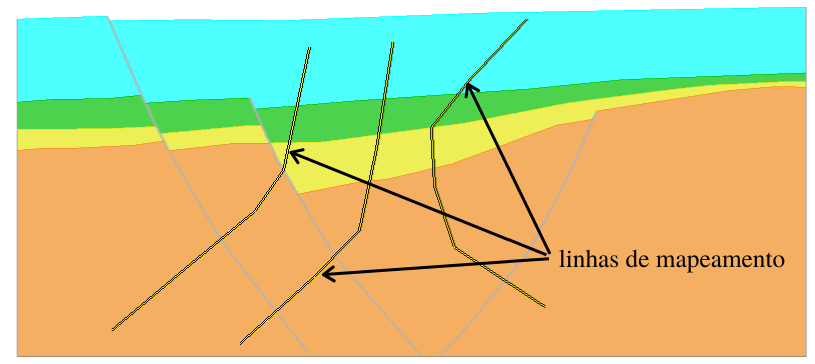
\includegraphics[width=400pt]{images/fig-linhas-de-mapeamento-ed}
    \caption{Linhas de mapeamento em uma seção.}\label{fig-linemap}
  \end{center}
\end{figure}

Cada face de uma seção tem como atributo uma malha triangulada, e as linhas de mapeamento são definidas no sistema de coordenadas local da malha de cada uma das faces. Além disso, é possível que uma linha de mapeamento cruze diversas malhas, por isso, a linha de mapeamento é definida como um conjunto de "partes" de linha de mapeamento, sendo cada parte pertencente a um trecho contínuo em uma mesma face. O processo de criação do mapeamento da linha é feito para cada parte. Na Figura~\ref{fig-linemap-malhas} é possível ver uma linha de mapeamento cortando algumas malhas diferentes.

\begin{figure} [h]
  \begin{center}
    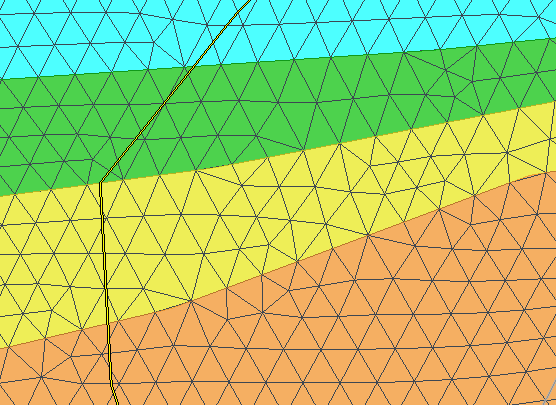
\includegraphics[width=350pt]{images/fig-linhas-de-mapeamento-malhas}
    \caption{Linhas de mapeamento cortando múltiplas faces.}\label{fig-linemap-malhas}
  \end{center}
\end{figure}

A primeira etapa desse mapeamento é a criação da linha-guia, a partir disso é feita a separação nas partes a serem processadas. É realizado um mapeamento com informações topológicas da interseção da parte com a malha. Essa ação consiste em fazer uma relação entre um ponto da parte da linha-guia e um ponto em uma entidade topológica da malha.

Por exemplo, na Figura~\ref{fig-linemap-parts} estão evidenciadas as partes que formam a linha de mapeamento. Cada uma dessas partes é representada pela entidade chamada \textit{LineMapPart}.

\begin{figure} [h]
  \begin{center}
    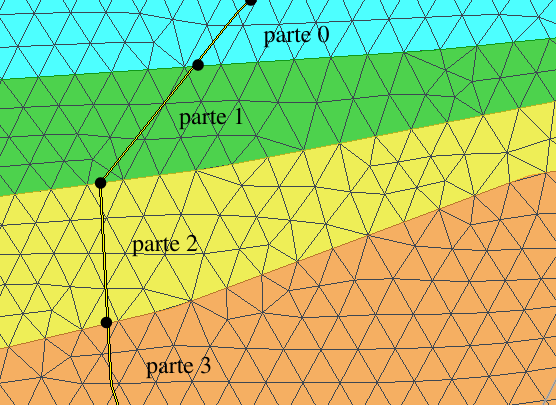
\includegraphics[width=350pt]{images/lm-parts}
    \caption{Partes de uma linha de mapeamento}\label{fig-linemap-parts}
  \end{center}
\end{figure}

